\index{cycle!thermodynamique|(textbf}
\section{Conventions graphiques}
\label{ch_conventions_graphiques}

	Nous commençons par nous accorder sur quelques conventions graphiques et de notation, qui sont résumées en \cref{fig_conventions_graphiques_travail_net}.
	
	\begin{figure}
		\begin{center}
			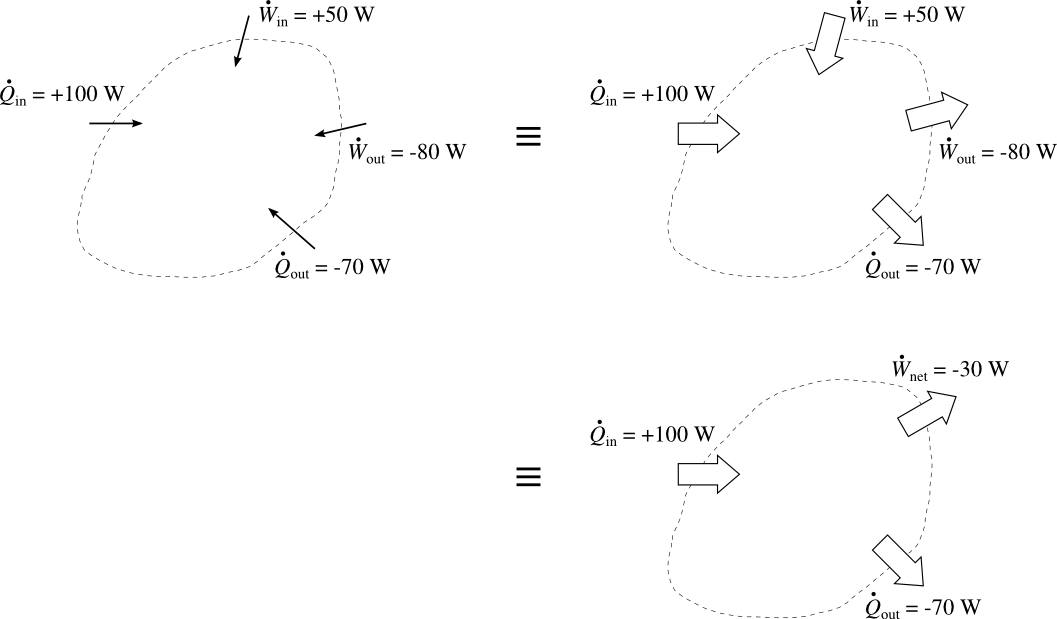
\includegraphics[width=\textwidth]{images/conventions_graphiques_travail_net.png}
		\end{center}
		\supercaption{Nouvelles conventions graphiques et de notation des transferts énergétiques.
			Les flèches blanches sont orientées selon le sens physique des transferts ; La somme algébrique de tous les travaux est représentée par un unique transfert nommé \vocab[travail!net]{travail net}.}{schéma \cczero \oc}
		\label{fig_conventions_graphiques_travail_net}
	\end{figure}

	Nous utilisons de larges flèches blanches pour représenter \emph{le sens physique des transferts}. Nous ne modifions pas notre convention de signe (les transferts sont positifs vers le système et négatifs lorsqu’ils en proviennent), mais seulement la convention graphique pour les orienter, afin de rendre la visualisation des transferts dans les machines plus intuitive.

	\index{puissance!nette}\index{énergie!transfert net}
	La somme algébrique du travail reçu $W_\inn$ et fourni $W_\out$ par une machine est nommé le \vocab[travail!net]{travail net} $W_\net$. Le travail net peut être positif (reçu par la machine de l’extérieur) ou négatif (fourni par la machine à l’extérieur), selon le type d’\mbox{application}.
	\begin{IEEEeqnarray}{rCl}
		W_\net 			& \equiv & W_\inn + W_\out 					\nonumber \\
		\dot W_\net 	& \equiv & \dot W_\inn + \dot W_\out 	\nonumber \\
		w_\net 			& \equiv & w_\inn + w_\out
	\label{def_travail_net}
	\end{IEEEeqnarray}

	On définit la \vocab[chaleur!nette]{chaleur nette} de la même façon :
	\begin{IEEEeqnarray}{rCl}
		Q_\net 			& \equiv & Q_\inn + Q_\out	 				\nonumber \\
		\dot Q_\net 	& \equiv & \dot Q_\inn + \dot Q_\out	\nonumber \\
		q_\net 			& \equiv & q_\inn + q_\out
	\end{IEEEeqnarray}

	Ainsi, par exemple, un moteur automobile reçoit une chaleur nette positive et produit un travail net négatif.
	\onlyframabook{\dontbreakpage}%handmade (pour éviter un saut de page zarbi)

\section{Transformer chaleur et travail}

	\subsection{Construire des cycles thermodynamiques}
	\label{ch_construction_cycle}\index{cycle!thermodynamique}

		Nous souhaitons comparer différentes manières de transformer travail et chaleur. Pour que ces comparaisons soient valables, il faut que nous tenions toujours compte de \emph{toutes} les transformations subies par le fluide jusqu’à ce qu’il soit revenu à son état initial.

		Par exemple, il est aisé de refroidir une pièce avec une bouteille d’air comprimé (il suffit de faire travailler le fluide pendant sa détente pour que sa température chute) ; mais si nous voulons refroidir la pièce en continu, alors il nous faut aussi tenir compte de l’énergie nécessaire pour \emph{ramener} l’air dans la bouteille, à sa pression et température initiales, à la fin du processus.
		
		Un second exemple est celui d’un moteur automobile, qui rejette de la chaleur emportée par les gaz d’échappement. Pour tenir compte de cette énergie perdue, nous comptabilisons la chaleur qu’il faudrait prélever aux gaz pour les ramener à la température d’entrée du moteur. Ce refroidissement imaginaire a lieu en dehors du moteur en pratique, mais d’un point de vue thermodynamique, il fait partie intégrante du processus de transformation énergétique.

		Ainsi, à chaque fois que nous allons analyser le fonctionnement d’une machine thermique, nous allons prendre soin de poursuivre l’évolution du fluide jusqu’à le ramener à son état initial (même température, même pression, même énergie interne, etc.). Nous disons alors qu’il a parcouru un \vocab[cycle!thermodynamique]{cycle thermodynamique} (\S\ref{ch_premier_principe_sf}).


	\subsection{Produire un travail à partir de chaleur}
	\label{ch_principe_fonctionnement_moteur}\index{moteur!principe de fonctionnement}

		Commençons par comprimer un fluide : nous augmentons sa pression et réduisons son volume spécifique, ce qui nous demande un certain travail. Après cela, chauffons ce fluide : sa pression et son volume ont tendance à augmenter. En détendant le fluide jusqu’à sa pression initiale, nous allons récupérer un travail plus grand que celui que nous avons investi à l’aller. Pour pouvoir enfin ramener le fluide à son état initial, il faut le refroidir.

		Au final, le fluide a dépensé moins de travail au chemin retour qu’il n’en a reçu à l’aller. Sur un cycle, il aura donc \emph{produit} du travail et absorbé (plus exactement, \emph{transformé}) de la chaleur. C’est le principe de fonctionnement d’un moteur.

		Il y a une infinité de cycles possibles pour effectuer cette transformation, mais ils comportent tous au moins quatre transferts énergétiques : une compression, un réchauffement, une détente et un refroidissement. Nous pouvons séparer ces évolutions dans l’espace, comme représenté en \cref{fig_cycle_thermodynamique_du_moteur_so}, ou bien dans le temps, comme montré en \cref{fig_cycle_thermodynamique_du_moteur_sf}. En fonction des contraintes technologiques et pratiques, certains de ces transferts peuvent être effectués simultanément.

		\onlyamphibook{\begin{figure}}
		\onlyframabook{\begin{figure}[h!]}
			\begin{center}
				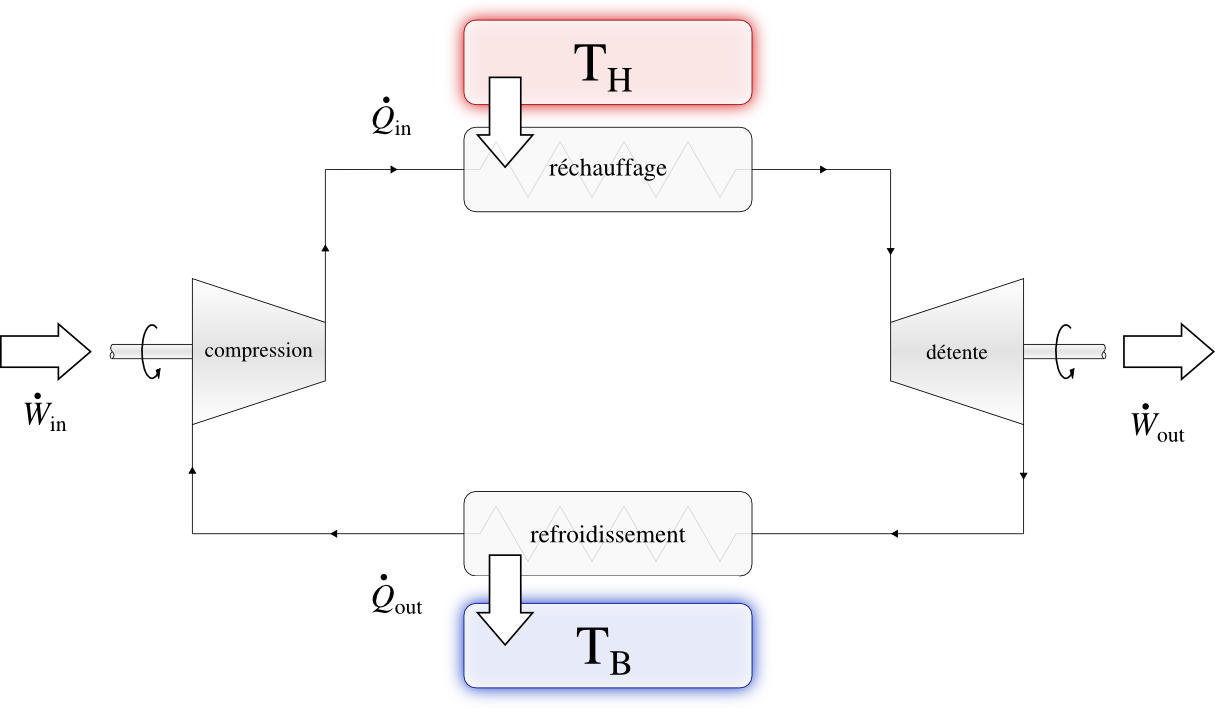
\includegraphics[width=\textwidth]{images/moteur_so.png}
			\end{center}
			\supercaption{Cycle thermodynamique moteur.
				Le fluide absorbe de la chaleur fournie à haute température $T_H$. la puissance de compression est plus faible que la puissance à la détente : la puissance nette sous forme de travail $\dot W_\net = \dot W_\inn + \dot W_\out$ est négative.}{schéma \cczero \oc}
			\label{fig_cycle_thermodynamique_du_moteur_so}
		\end{figure}

		\onlyamphibook{\begin{figure}}
		\onlyframabook{\begin{figure}[h!]}
			\begin{center}
				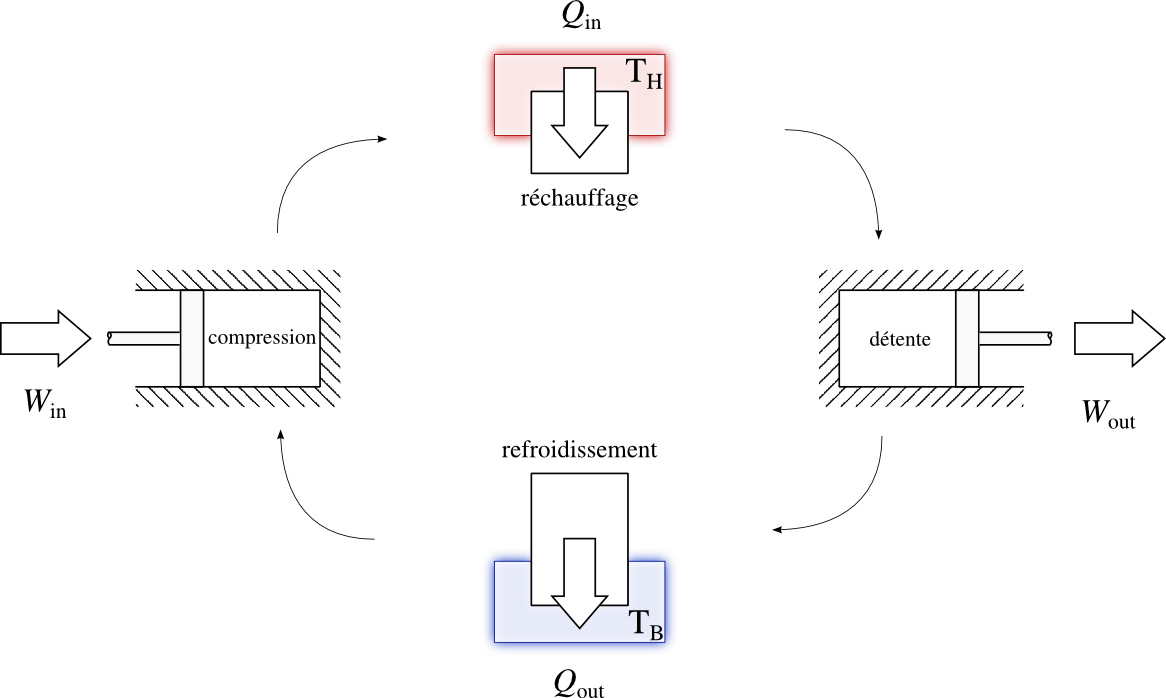
\includegraphics[width=\textwidth]{images/moteur_sf.png}
			\end{center}
			\supercaption{Cycle thermodynamique moteur effectué en séparant les étapes dans le temps (plutôt que dans l’espace comme représenté en \cref{fig_cycle_thermodynamique_du_moteur_so}). Le fluide est réchauffé par une source de chaleur à haute température $T_H$. Le travail net $W_\net = W_\inn + W_\out$ est négatif.}{schéma \cczero \oc}
			\label{fig_cycle_thermodynamique_du_moteur_sf}
		\end{figure}

		Il est possible de lier mécaniquement les sections consommant et fournissant de l’énergie sous forme de travail. Dans le cas où le fluide circule en continu, on peut lier le compresseur et la turbine par un même axe, comme représenté en \cref{fig_cycle_thermodynamique_du_moteur_axe_so}. Dans le cas où les évolutions sont séparées dans le temps, comme dans un moteur à explosion, on peut lier les évolutions en effectuant plusieurs cycles déphasés simultanément (avec plusieurs cylindres) ou en stockant de l’énergie dans un volant d’inertie. Le moteur ne reçoit alors pas de travail extérieur et on obtient alors à sa sortie une puissance $\dot W_\net$.

		\onlyamphibook{\begin{figure}}
		\onlyframabook{\begin{figure}[h!]}
			\begin{center}
				\onlyamphibook{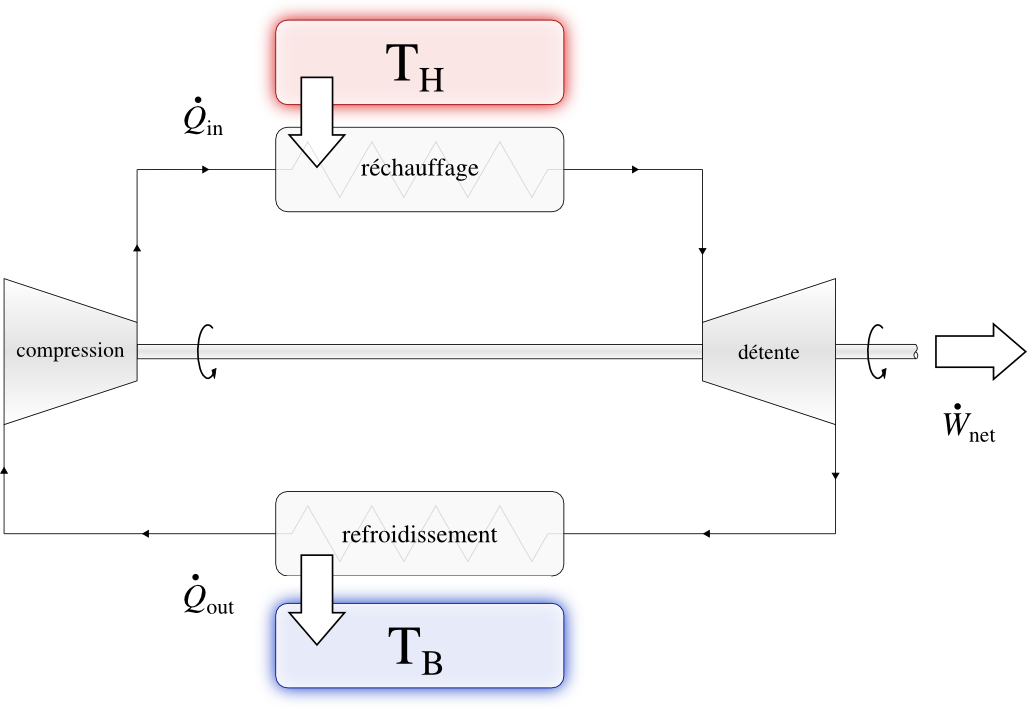
\includegraphics[width=\textwidth]{images/moteur_so_travail_net.png}}
				\onlyframabook{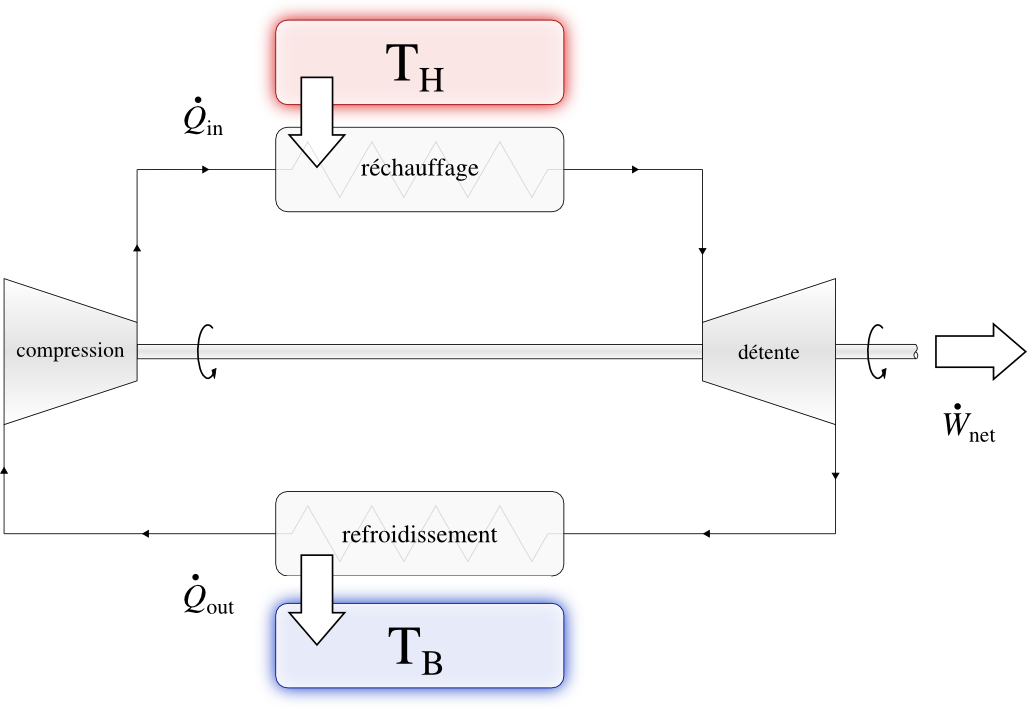
\includegraphics[width=0.8\textwidth]{images/moteur_so_travail_net.png}}
			\end{center}
			\supercaption{Cycle thermodynamique moteur, pour lequel le compresseur et la turbine sont reliés mécaniquement. Comme la turbine fournit une puissance $\dot W_\out$ supérieure à celle consommée par le compresseur ($\dot W_\inn$), elle est capable non seulement de l’entraîner mais aussi de fournir un excédent $\dot W_\net$ vers l’extérieur.}{schéma \cczero \oc}
			\label{fig_cycle_thermodynamique_du_moteur_axe_so}
		\end{figure}


	\subsection{Extraire de la chaleur avec du travail}
	\label{ch_principe_fonctionnement_réfrigérateur}\index{réfrigérateur!principe de fonctionnement|(textbf}\index{pompe à chaleur!principe de fonctionnement|(textbf}\index{climatiseur!principe de fonctionnement|(textbf}\index{chaleur!transfert vers une température plus haute}\index{cycle!de réfrigération (ou climatisation)}

			Lorsque l’on fournit du travail à un fluide, sa température augmente\footnote{Ce n’est pas strictement vrai pour les liquides/vapeurs qui, comme nous l’avons vu dans le \courscinq, connaissent une phase à température constante entre leurs points de saturation – toutefois, ils suivent cette tendance générale hors de cette plage de propriétés.} et il peut ainsi fournir de la chaleur à un corps qui était initialement à plus haute température («~plus chaud~») que lui.

			À l’inverse, lorsque l’on détend un fluide, sa température baisse et il peut ainsi capter de la chaleur à un corps qui était initialement «~plus froid~» que lui.

			En effectuant ces étapes l’une après l’autre, nous obtenons un \vocab[cycle!de réfrigération (ou climatisation)]{cycle de \mbox{réfrigération}} : une machine capable de prélever de la chaleur à basse température et de la rejeter à haute température. Un tel cycle est représenté en \cref{fig_refrigerateur_climatiseur_thermopompe_so} (étapes séparées dans l’espace) et \ref{fig_refrigerateur_climatiseur_thermopompe_sf} (étapes séparées dans le temps).
			
			Un examen attentif de ces deux figures réserve une surprise de taille : il s’agit exactement du même agencement que pour un moteur ! La seule différence porte sur les températures de fonctionnement. La température atteinte pendant la compression doit être \textbf{supérieure à la température haute $T_H$}, et la température atteinte pendant la détente doit être \textbf{inférieure à la température basse $T_B$}. Si ces conditions ne sont pas respectées, alors les transferts de chaleur ne peuvent pas se faire dans le sens voulu.
			
			\begin{figure}
				\begin{center}
					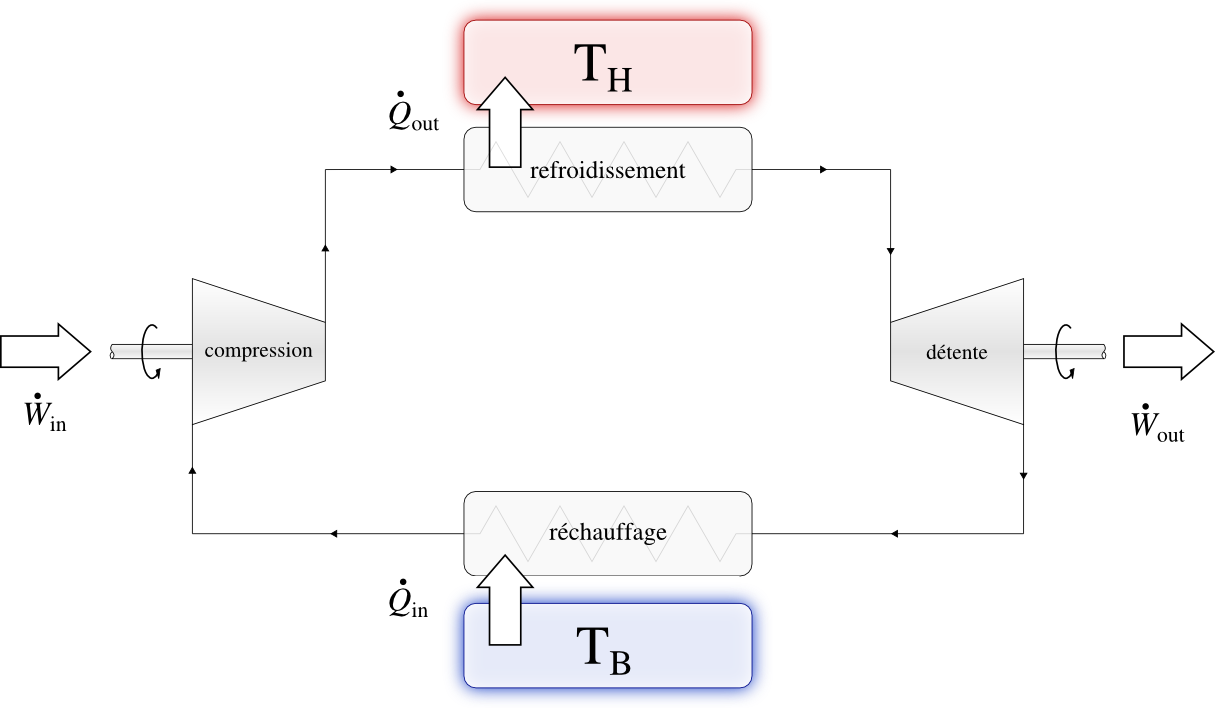
\includegraphics[width=\textwidth]{images/refrigerateur_climatiseur_thermopompe_so.png}
				\end{center}
				\supercaption{Cycle thermodynamique de refroidissement, utilisé dans les réfrigérateurs, climatiseurs et pompes à chaleur.\\
					Une puissance $\dot Q_\inn$ sous forme de chaleur est captée à basse température (le fluide est réchauffé) tandis qu’une puissance $\dot Q_\out$ est rejetée à haute température (le fluide est alors refroidi).}{schéma \cczero \oc}
				\label{fig_refrigerateur_climatiseur_thermopompe_so}
			\end{figure}

			\begin{figure}
				\begin{center}
					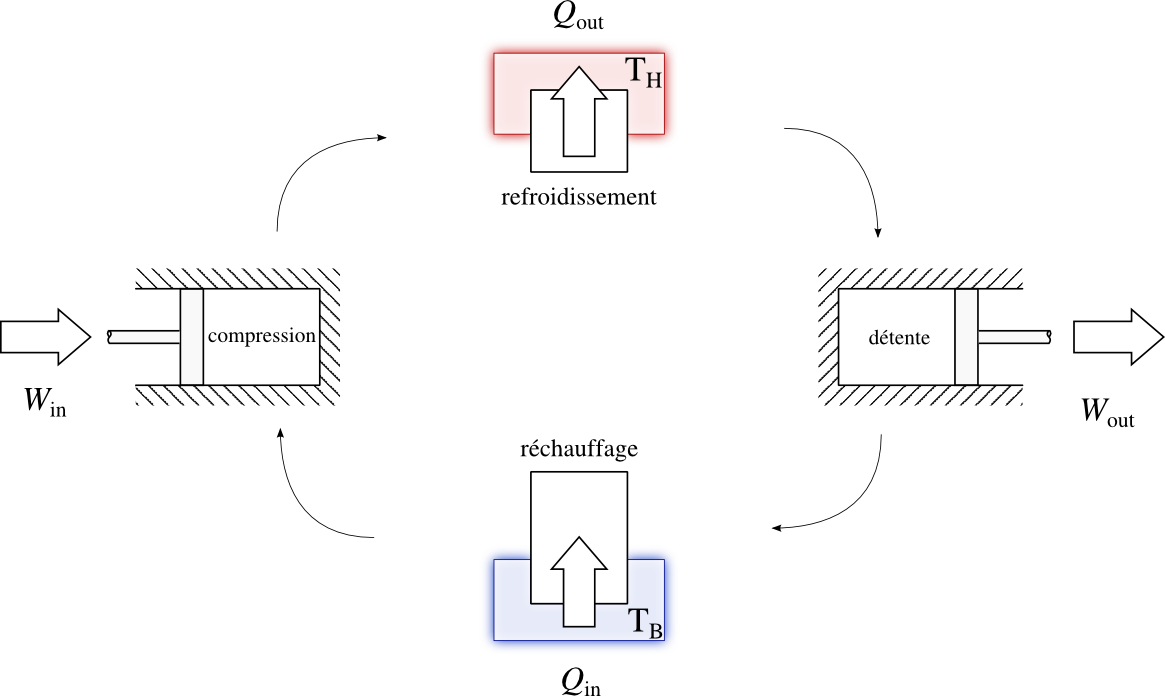
\includegraphics[width=\textwidth]{images/refrigerateur_climatiseur_thermopompe_sf.png}
				\end{center}
				\supercaption{Cycle de réfrigération effectué en séparant les étapes dans le temps (plutôt que dans l’espace comme représenté en \cref{fig_refrigerateur_climatiseur_thermopompe_so})}{schéma \cczero \oc}
				\label{fig_refrigerateur_climatiseur_thermopompe_sf}
			\end{figure}

			Dans un cycle de réfrigération, le fluide a un plus grand volume lorsqu’il est compressé (après avoir été réchauffé) que lorsqu’il est détendu (après avoir été refroidi) : cette fois la compression demande plus de puissance que la détente. La puissance nette $\dot W_\net$ sous forme de travail est donc positive, c’est-à-dire que la machine doit être alimentée en travail par l’extérieur.

			En pratique dans les systèmes de réfrigération, on a souvent recours à une astuce pour faire chuter la température : au lieu d’une turbine, on utilise une simple soupape (parfois appelée \vocab{détendeur}). Cet élément sans pièce mobile ne permet pas de dégager de travail (il augmente donc la puissance consommée par la machine), mais il est beaucoup plus simple de fabrication et d’utilisation.

			\index{Joule!détente de Gay-Lussac et}\index{Gay-Lussac!détente de Joule et}\index{travail!lors des irréversiblités}
			La soupape, en termes thermodynamiques, permet d’effectuer une détente entièrement irréversible, augmentant le volume et baissant la pression sans extraire de travail. Si l’on utilisait un gaz parfait, cela n’aurait aucun effet sur la température\footnote{Revoir à ce propos les expériences de Joule et Gay-Lussac étudiées en \S\ref{ch_principe_de_joule} p.\pageref{ch_principe_de_joule}.} et donc aucun intérêt ; mais lorsque l’on utilise des liquides/vapeurs, la détente en soupape est un moyen technologiquement simple de faire chuter la température. Cette modification est décrite en \cref{fig_principe_du_réfrigérateur_soupape}.

		\onlyamphibook{\begin{figure}}
		\onlyframabook{\begin{figure}[h!]}
				\begin{center}
					\onlyamphibook{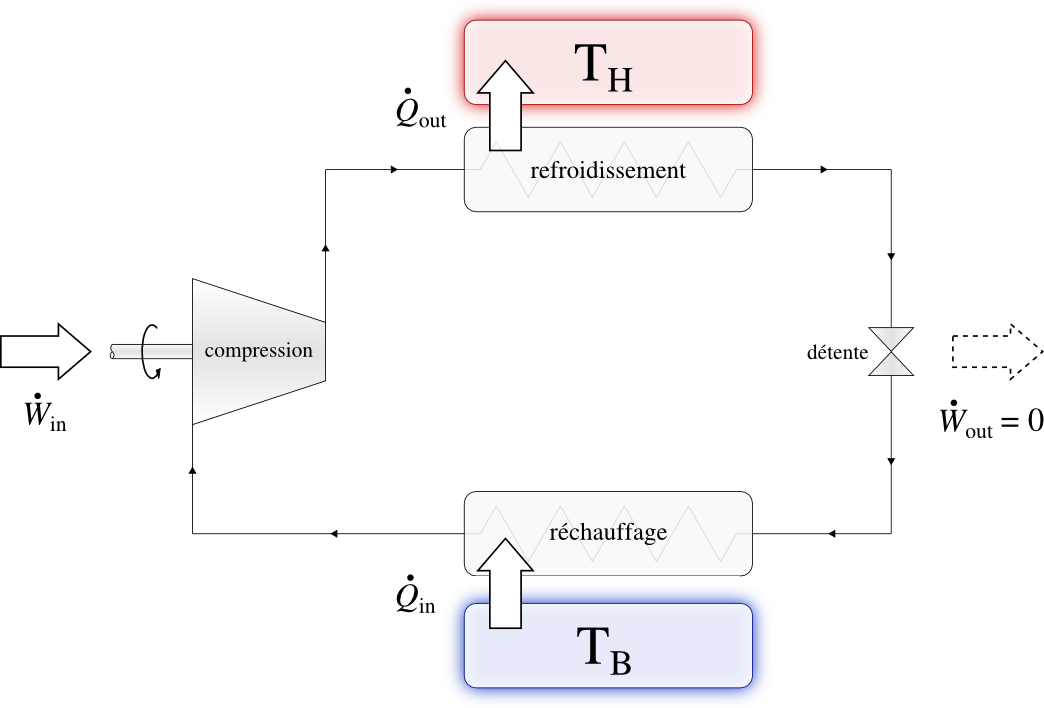
\includegraphics[width=\textwidth]{images/refrigerateur_climatiseur_thermopompe_so_soupape.png}}
					\onlyframabook{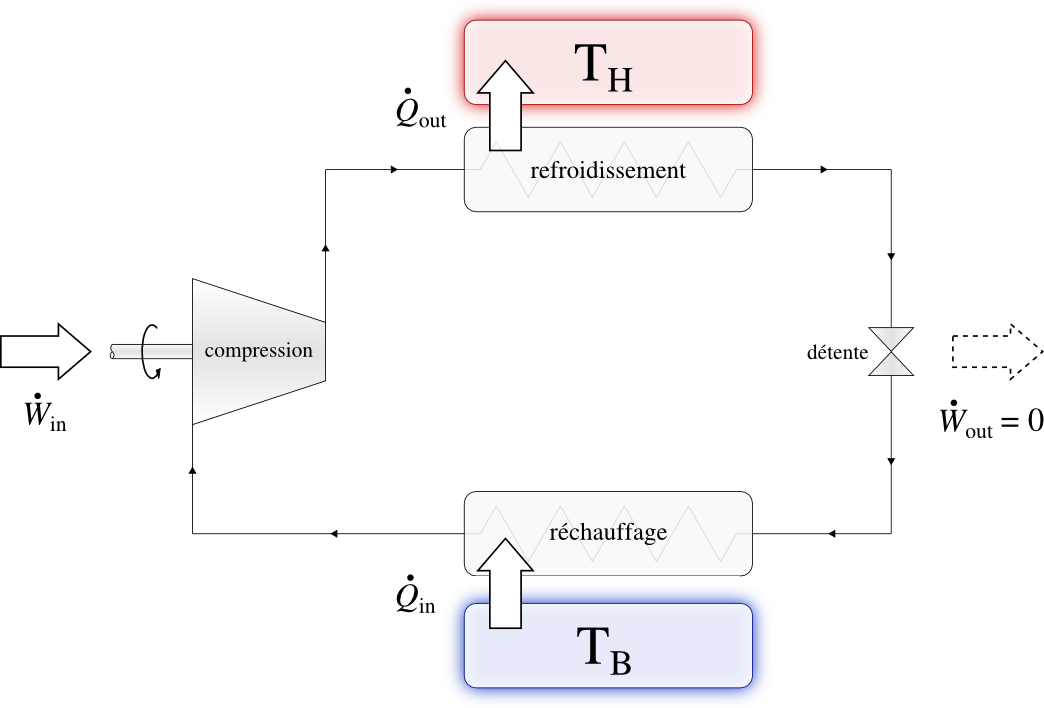
\includegraphics[width=0.8\textwidth]{images/refrigerateur_climatiseur_thermopompe_so_soupape.png}}
				\end{center}
				\supercaption{Cycle de réfrigération modifié.
					Lorsque l’on utilise des liquides/vapeurs, il est possible de se dispenser d’extraire du travail lors de la détente. L’utilisation d’une simple soupape suffit pour faire baisser la température du fluide.}{schéma \cczero \oc}
				\label{fig_principe_du_réfrigérateur_soupape}
			\end{figure}

			\clearfloats\onlyframabook{\clearpage}
			Les cycles de réfrigération ont deux grands types d’application :
			\begin{description}
				\item[Les pompes à chaleur]\index{pompe à chaleur} appelées aussi \vocab[pompe à chaleur]{thermopompes} (\cref{fig_agencement_thermopompe}) sont agencées de façon à rejeter la chaleur vers un corps à haute température, le plus souvent une habitation ;
				\item[Les réfrigérateurs et climatiseurs]\index{réfrigérateur}\index{climatiseur} (\cref{fig_agencement_refrigerateur_climatiseur}) sont agencés de façon à extraire de la chaleur d’un corps à basse température, le plus souvent une chambre froide.
			\end{description}

		\onlyamphibook{\begin{figure}}
		\onlyframabook{\begin{figure}[h!]}
				\begin{center}
					\onlyamphibook{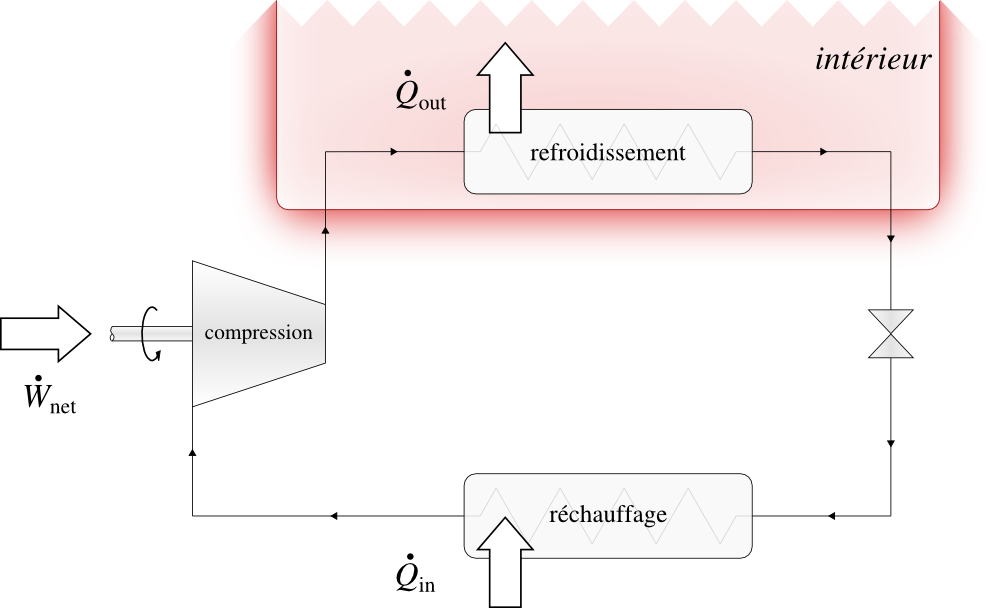
\includegraphics[width=\textwidth]{images/agencement_thermopompe.png}}
					\onlyframabook{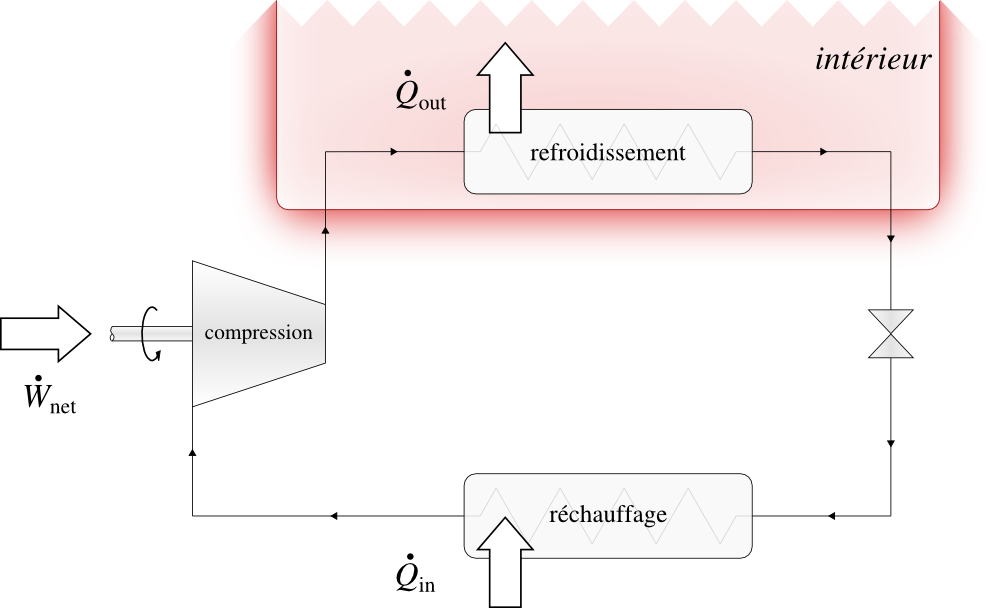
\includegraphics[width=0.8\textwidth]{images/agencement_thermopompe.png}}
				\end{center}
				\supercaption{Agencement d’une pompe à chaleur. La machine est positionnée de sorte à refouler à l’intérieur (où la température est plus haute) la chaleur prélevée à l’extérieur (où la température est plus basse).}{schéma \cczero \oc}
				\label{fig_agencement_thermopompe}
			\end{figure}
			
		\onlyamphibook{\begin{figure}}
		\onlyframabook{\begin{figure}[h!]}
				\begin{center}
					\onlyamphibook{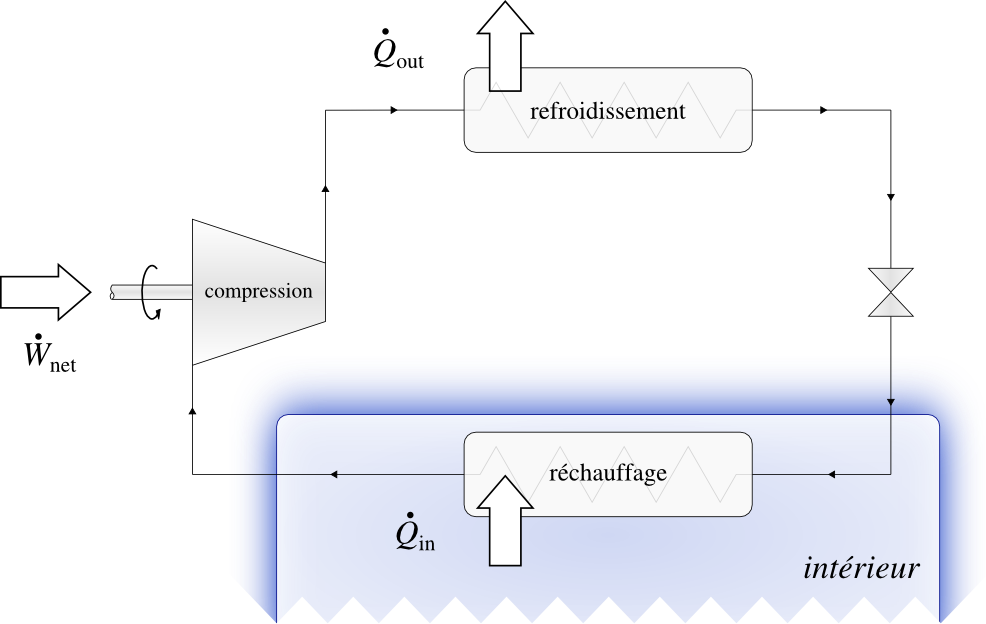
\includegraphics[width=\textwidth]{images/agencement_refrigerateur_climatiseur.png}}
					\onlyframabook{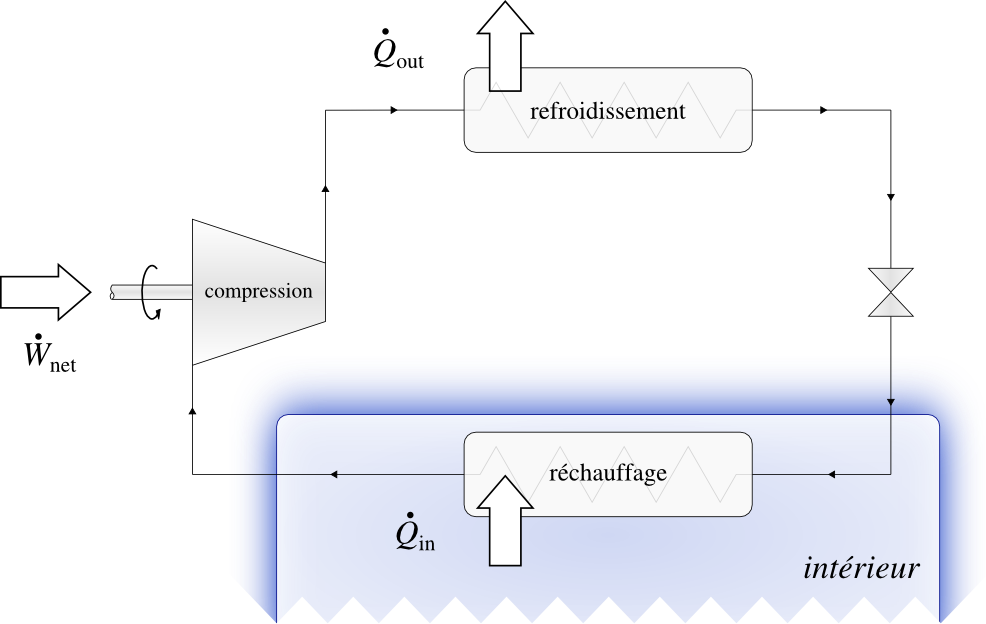
\includegraphics[width=0.8\textwidth]{images/agencement_refrigerateur_climatiseur.png}}
				\end{center}
				\supercaption{Agencement d’un réfrigérateur ou d’un climatiseur. La machine est positionnée de sorte à refouler à l’extérieur (où la température est plus haute) la chaleur prélevée à l’intérieur (où la température est plus basse). Il s’agit exactement de la même machine qu’en \cref{fig_agencement_thermopompe}.}{schéma \cczero \oc}
				\label{fig_agencement_refrigerateur_climatiseur}
			\end{figure}

			Dans ces deux types d’application, il s’agit exactement de la même machine, fonctionnant avec le même cycle. La seule différence concerne l’agencement intérieur/extérieur des composants : une pompe à chaleur n’est ni plus ni moins qu’un réfrigérateur positionné de sorte qu’il «~refroidisse l’extérieur~».

			\clearfloats
			La similarité entre climatiseur et pompe à chaleur permet d’effectuer ces deux fonctions avec une seule même machine, que l’on dit alors \vocab[inversable vs. réversible]{inversable} – ou parfois \vocab[réversibilité!réversible vs. inversable]{réversible}, à tort comme nous le verrons au \courssept. En fonction des besoins, le sens de circulation du fluide est inversé, ce qui provoque l’inversion des transferts de chaleur. Ce type de machine est représenté en \cref{fig_agencement_thermopompe_climatiseur_inversable}.
			
			\onlyframabook{\begin{figure}[htc]}
			\onlyamphibook{\begin{figure}}%handmade
				\begin{center}
					\onlyamphibook{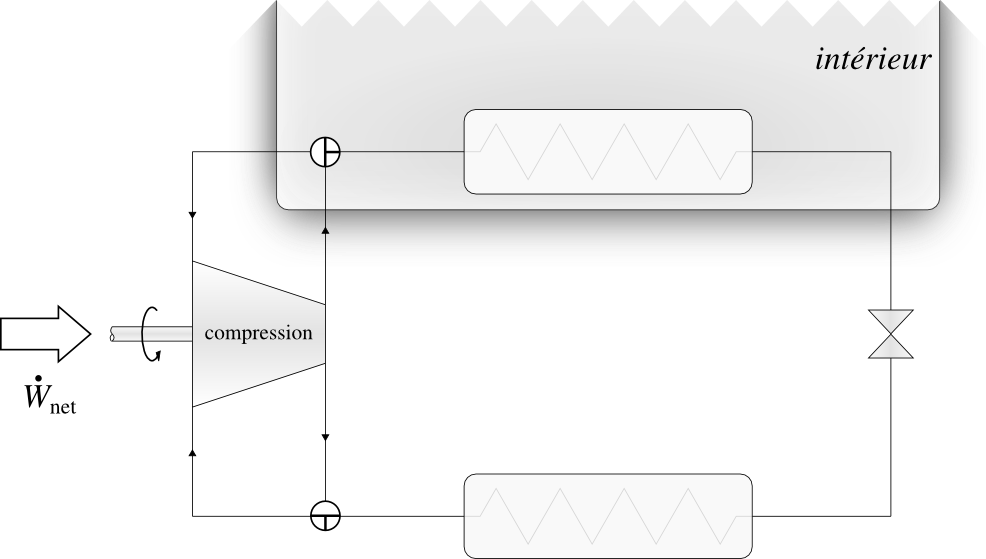
\includegraphics[width=\textwidth]{images/agencement_thermopompe_climatiseur_inversable.png}}
					\onlyframabook{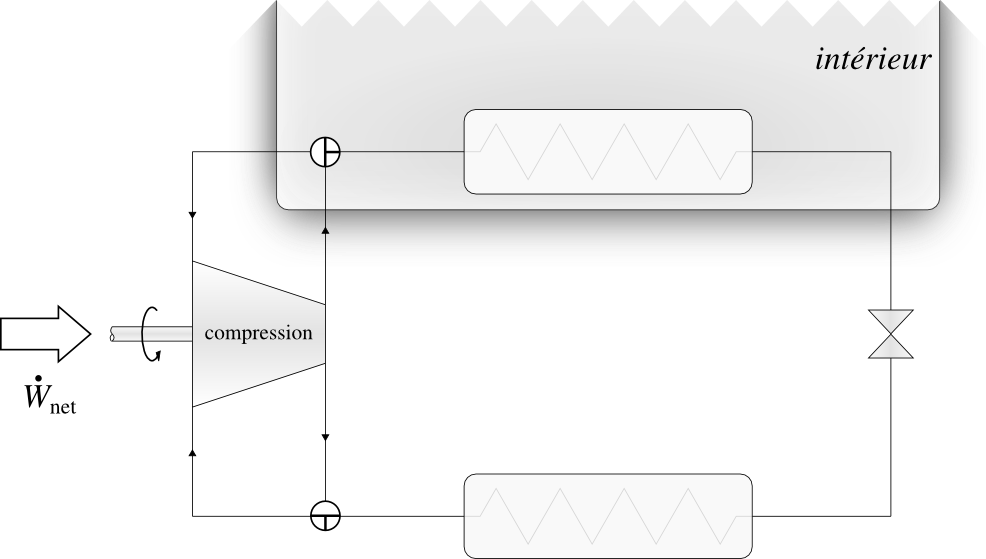
\includegraphics[width=0.8\textwidth]{images/agencement_thermopompe_climatiseur_inversable.png}}
				\end{center}
				\supercaption{Agencement d’un climatiseur inversable. En pivotant des deux vannes de~\SI{90}{\degree} dans le sens anti-horaire, on change la fonction depuis une pompe à chaleur vers un climatiseur.}{schéma \cczero \oc}
				\label{fig_agencement_thermopompe_climatiseur_inversable}
			\end{figure}
		\index{réfrigérateur!principe de fonctionnement|)textbf}\index{pompe à chaleur!principe de fonctionnement|)textbf}\index{climatiseur!principe de fonctionnement|)textbf}

\section{Rendement des cycles}

	Le \vocab{rendement}\footnote{Dans le présent ouvrage, nous utilisons indistinctement les termes \textit{efficacité} et \textit{rendement}. Toutefois, certains auteurs font une distinction entre l’efficacité $\eta$ définie en~\ref{def_efficacité_machines_thermiques} et un rendement $R \equiv \frac{\eta_\text{réele}}{\eta_\text{théorique}}$ comparant l’efficacité atteinte en pratique avec l’efficacité maximale atteignable par la machine. Il faut alors soigneusement défnir les hypothèses associées au calcul de l’efficacité maximale.}%
	 ou l’\vocab{efficacité} $\eta$ d’une machine thermique compare le transfert ou la transformation utile qu’elle effectue avec le coût énergétique qu’elle engendre. Nous retiendrons la définition de principe suivante :
	\begin{equation}
		\eta \equiv \left| \frac{\text{transfert utile}}{\text{dépense énergétique}} \right|
		\label{def_efficacité_machines_thermiques}
	\end{equation}

	Par convention le rendement est toujours exprimé sous la forme d’un nombre positif ; ainsi nous utilisons une valeur absolue dans l’\cref{def_efficacité_machines_thermiques}. Pour chacun des trois types de machines thermiques, nous allons définir et quantifier ce «~transfert utile~» et cette «~dépense énergétique~».


	\subsection{Rendement d’un moteur}
	\label{ch_rendement_moteur}\index{moteur!rendement d’un}\index{efficacité!d’un moteur}

		La fonction d’un moteur thermique, comme ceux que l’on trouve à bord des automobiles ou dans les centrales électriques, est de produire du travail, c’est-à-dire une quantité $\dot W_\net$ négative (\cref{fig_transferts_moteur}). La dépense engendrée pour générer ce travail est la chaleur qu’il reçoit, c’est-à-dire la quantité $\dot Q_\inn$ (provenant usuellement de la combustion de carburant ou de la fission de noyaux atomiques).

		\onlyamphibook{\begin{figure}}
		\onlyframabook{\begin{figure}[h!]}
			\begin{center}
				\vspace{-0.5cm}
				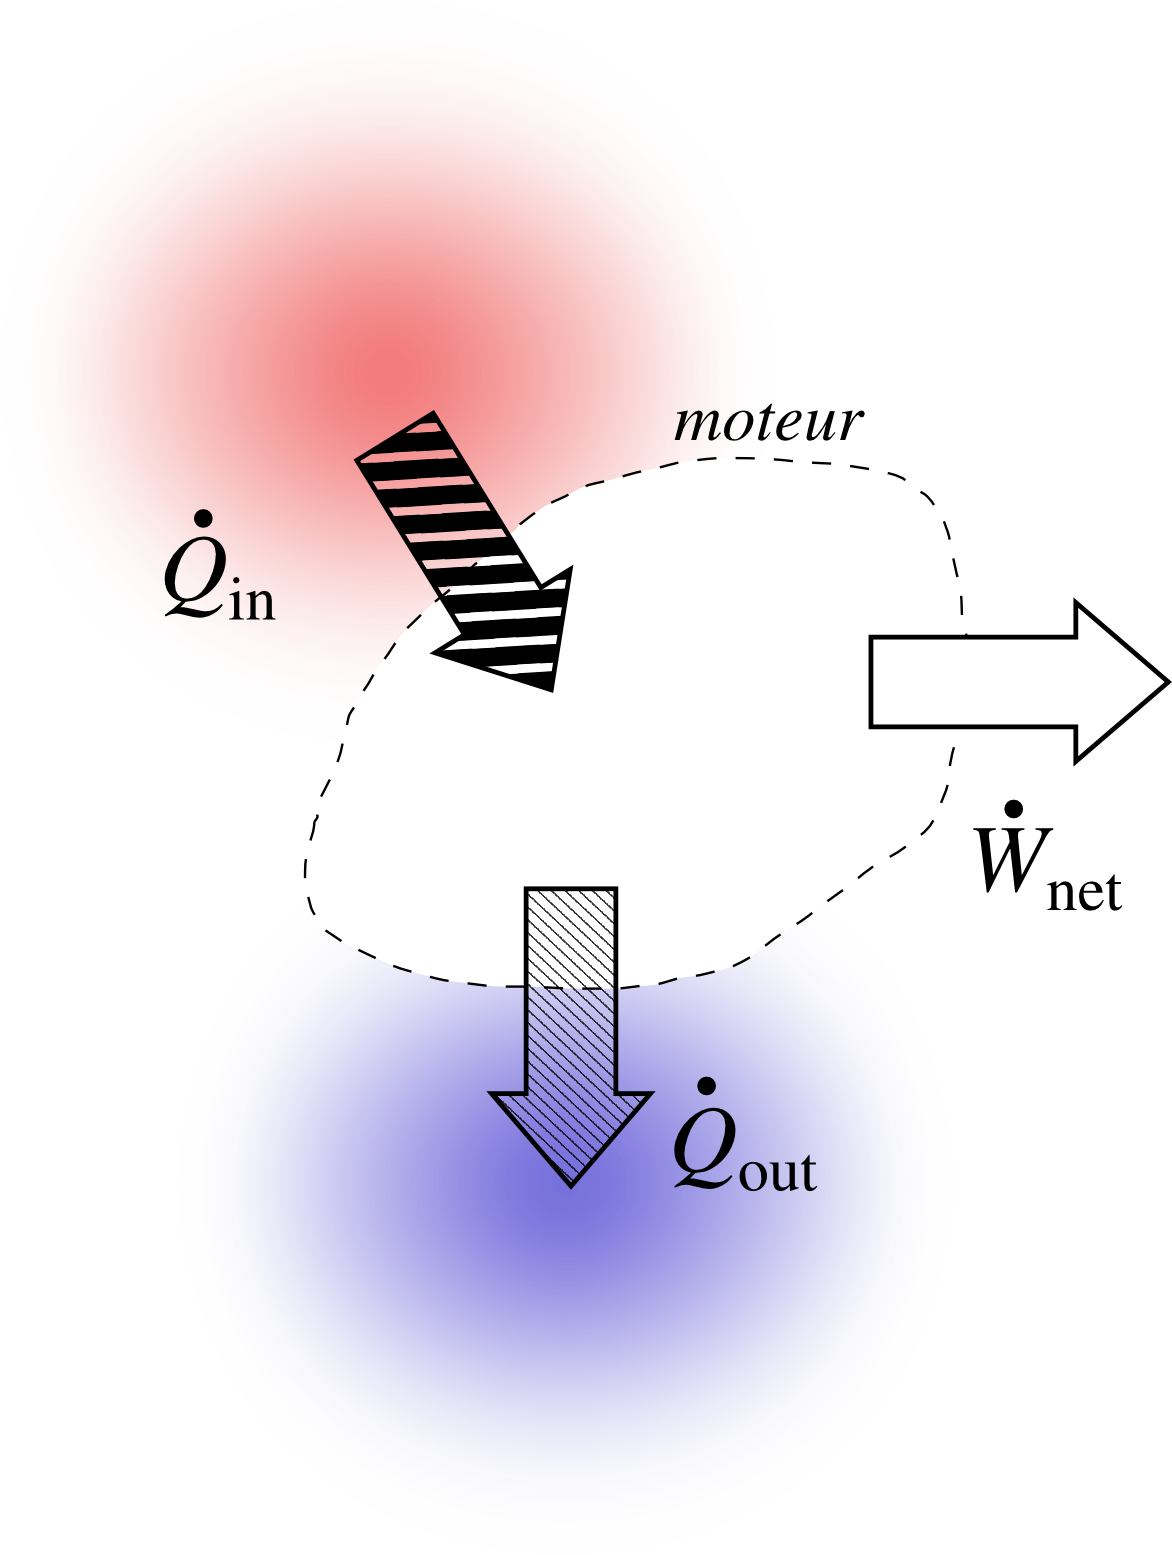
\includegraphics[width=6cm]{images/efficacite_moteur.png}
				\vspace{-1cm}
			\end{center}
			\supercaption{Transferts énergétiques associés à un moteur.
				On souhaite obtenir un grand transfert $\dot W_\net$  (résultat) à partir du transfert $\dot Q_\inn$ (coût).
				Le rejet $\dot Q_\out$ est indésirable.}{schéma \cczero \oc}
			\label{fig_transferts_moteur}
		\end{figure}

		D’après la définition~\ref{def_efficacité_machines_thermiques} le rendement $\eta_\text{moteur}$ du moteur thermique est donc :
		\begin{equation}
			\eta_\text{moteur} \equiv \left| \frac{\dot W_\net}{\dot Q_\inn} \right|
			\label{def_rendement_moteur}
		\end{equation}

		\begin{anexample}
			Un moteur automobile reçoit une puissance de~\SI{100}{\kilo\watt} sous forme de chaleur issue de la combustion d’essence ; il fournit \SI{55}{\kilo\watt} sous forme de travail à l’arbre de transmission. Quel est son rendement ?
	
			\begin{answer}
				Le rendement est de $\eta_\text{moteur} = \left| \frac{\dot W_\net}{\dot Q_\inn} \right| = \left| \frac{\num{-55e3}}{\num{+100e3}} \right| = \num{0,55} = \SI{55}{\percent}$.
					\begin{remark} Ce moteur effectue un rejet $\dot Q_\out = -\dot W_\net - \dot Q_\inn = -(\num{-55e3}) - \num{100e3}= \SI{-45}{\kilo\watt}$. Cette chaleur est en majeure partie évacuée par le pot d’échappement.\end{remark}
					\begin{remark} On se doute bien qu’il faudra toujours fournir au moins autant de chaleur $\dot Q_\inn$ que le moteur ne fournit de travail $\dot W_\net$ ; le rendement d’un moteur sera donc toujours nécessairement inférieur à~\num{1}.\end{remark}
			\end{answer}
		\end{anexample}

		La puissance nette $\dot W_\net$ sous forme de travail peut être exprimée en fonction des autres transferts énergétiques, et ainsi :
		\begin{IEEEeqnarray}{rCl}
			\dot W_\net 			& = & \dot W_\inn + \dot W_\out = -\dot Q_\inn - \dot Q_\out	\nonumber \\
			\eta_\text{moteur} 	& = & 1 - \left| \frac{\dot Q_\out}{\dot Q_\inn} \right|	\label{eq_rendement_moteur_qin_qout}
		\end{IEEEeqnarray}

		Cette \cref{eq_rendement_moteur_qin_qout} nous sera fort utile au chapitre prochain (\S\ref{ch_efficacité_moteur_carnot} p.\pageref{ch_efficacité_moteur_carnot}), où nous voudrons lier les transferts de chaleur $\dot Q_\inn$ et $\dot Q_\out$ aux températures auxquelles ils sont effectués.



	\subsection{Rendement d’un réfrigérateur ou d’un climatiseur}
	\label{ch_rendement_réfrigérateur}\index{climatiseur!rendement d’un}\index{réfrigérateur!rendement d’un}\index{efficacité!d’un climatiseur}\index{efficacité!d’un réfrigérateur}

		La fonction d’un réfrigérateur ou d’un climatiseur est d’extraire de la chaleur, c’est-à-dire de générer une puissance $\dot Q_\inn$ (chaleur extraite chaque seconde du compartiment à refroidir) de signe positif. Ce transfert (\cref{fig_transferts_réfrigérateur}) est rendu possible par l’apport au réfrigérateur d’un travail, $\dot W_\net$ , une «~dépense~» nécessairement~\mbox{positive}.

		\begin{figure}
			\begin{center}
				\vspace{-0.5cm}
				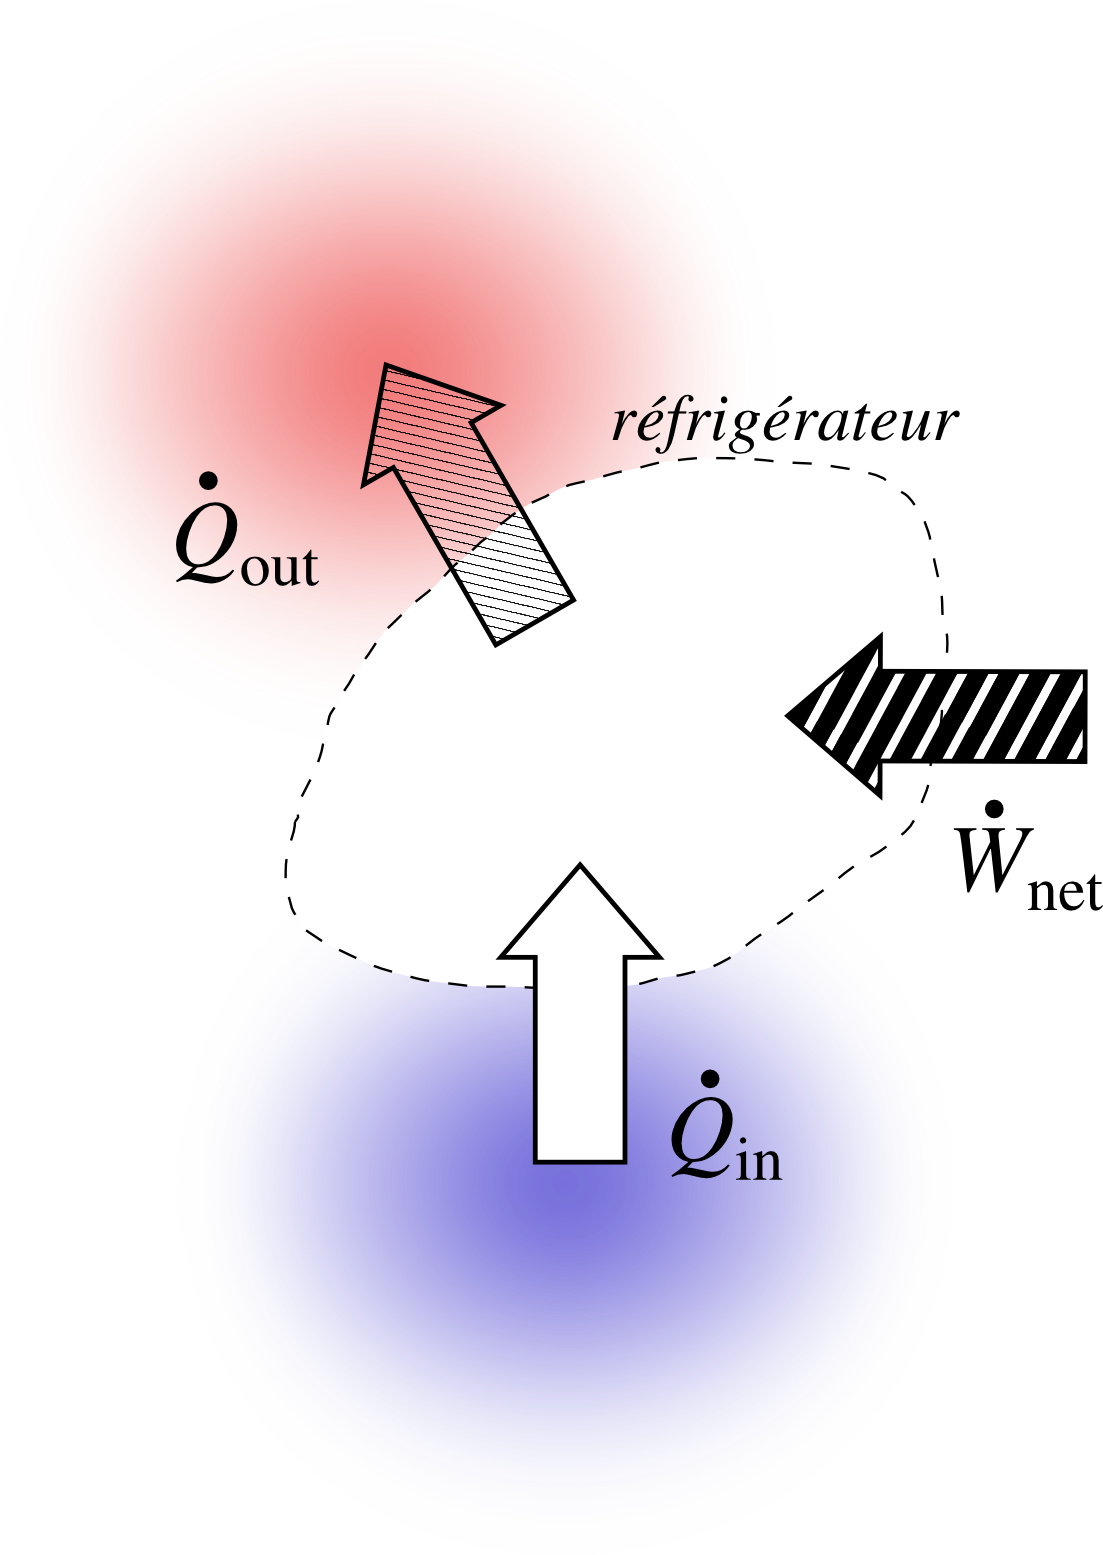
\includegraphics[width=6cm]{images/efficacite_refrigerateur_climatiseur.png}
				\vspace{-1cm}
			\end{center}
			\supercaption{Transferts énergétiques associés à un réfrigérateur ou à un climatiseur.
				On souhaite obtenir un grand transfert $\dot Q_\inn$ (résultat) à partir du transfert $\dot W_\net$ (coût).}{schéma \cczero \oc}
			\label{fig_transferts_réfrigérateur}
		\end{figure}

		D’après la définition~\ref{def_efficacité_machines_thermiques} le rendement (dit aussi parfois \vocab[coefficient of performance (COP)]{coefficient of performance}\index{COP (coefficient of performance)}, ou $\textsc{cop}_\text{réfrigération}$) d’un réfrigérateur ou d’un climatiseur est donc :
		\begin{equation}
			\eta_\text{réfrigérateur} = \eta _\text{climatiseur} \equiv \left| \frac{\dot Q_\inn}{\dot W_\net} \right|
			\label{def_rendement_climatiseur_refrigerateur}
		\end{equation}

		\onlyframabook{\clearfloats}
		\begin{anexample}
			Un réfrigérateur consomme une puissance électrique de~\SI{100}{\watt} ; il extrait de la chaleur de la chambre froide avec une puissance de~\SI{120}{\watt}. Quel est son rendement ?
	
			\begin{answer}
				Le rendement est de $\eta_\text{réfrigérateur} = \left| \frac{\dot Q_\inn}{\dot W_\net} \right| = \left| \frac{\num{+120}}{\num{+100}} \right| = \num{1,2} = \SI{120}{\percent}$.
					\begin{remark} Ce réfrigérateur effectue un rejet $\dot Q_\out = -\dot W_\net - \dot Q_\inn = \num{-100} - \num{120}= \SI{-220}{\watt}$ à l’extérieur de la chambre froide (usuellement, dans l’habitation elle-même).\end{remark}
					\begin{remark} Les réfrigérateurs et climatiseurs domestiques ont souvent un rendement supérieur à~\num{1} mais en fonction des températures demandées, le rendement peut tout à fait y être inférieur.\end{remark}
			\end{answer}
		\end{anexample}

		En prenant garde aux pièges algébriques associés à l’utilisation de valeurs absolues, pour préparer le chapitre prochain (\S\ref{ch_efficacite_refrigerateur_carnot} p.\pageref{ch_efficacite_refrigerateur_carnot}) nous pouvons exprimer ce rendement en fonction des transferts de chaleur uniquement :
		\begin{equation}
			\eta _\text{réfrigérateur} = \eta _\text{climatiseur} = \frac{1}{\left| \frac{\dot Q_\out}{\dot Q_\inn} \right| - 1}
			\label{rendement_réfrigérateur_qin_qout}
		\end{equation}





	\subsection{Rendement d’une pompe à chaleur}
	\label{ch_rendement_thermopompe}\index{pompe à chaleur!rendement d’une}\index{efficacité!d’une pompe à chaleur}

		Une pompe à chaleur fonctionne exactement de la même manière qu’un climatiseur. Sa fonction est de générer un transfert $\dot Q_\out$ vers la section «~chaude~» (usuellement l’intérieur d’une habitation). Ce transfert, représenté en \cref{fig_transferts_thermopompe}, est rendu possible par l’apport à la thermopompe de $\dot W_\net$ , une «~dépense~» nécessairement positive.

		\begin{figure}
			\begin{center}
				\vspace{-0.5cm}
				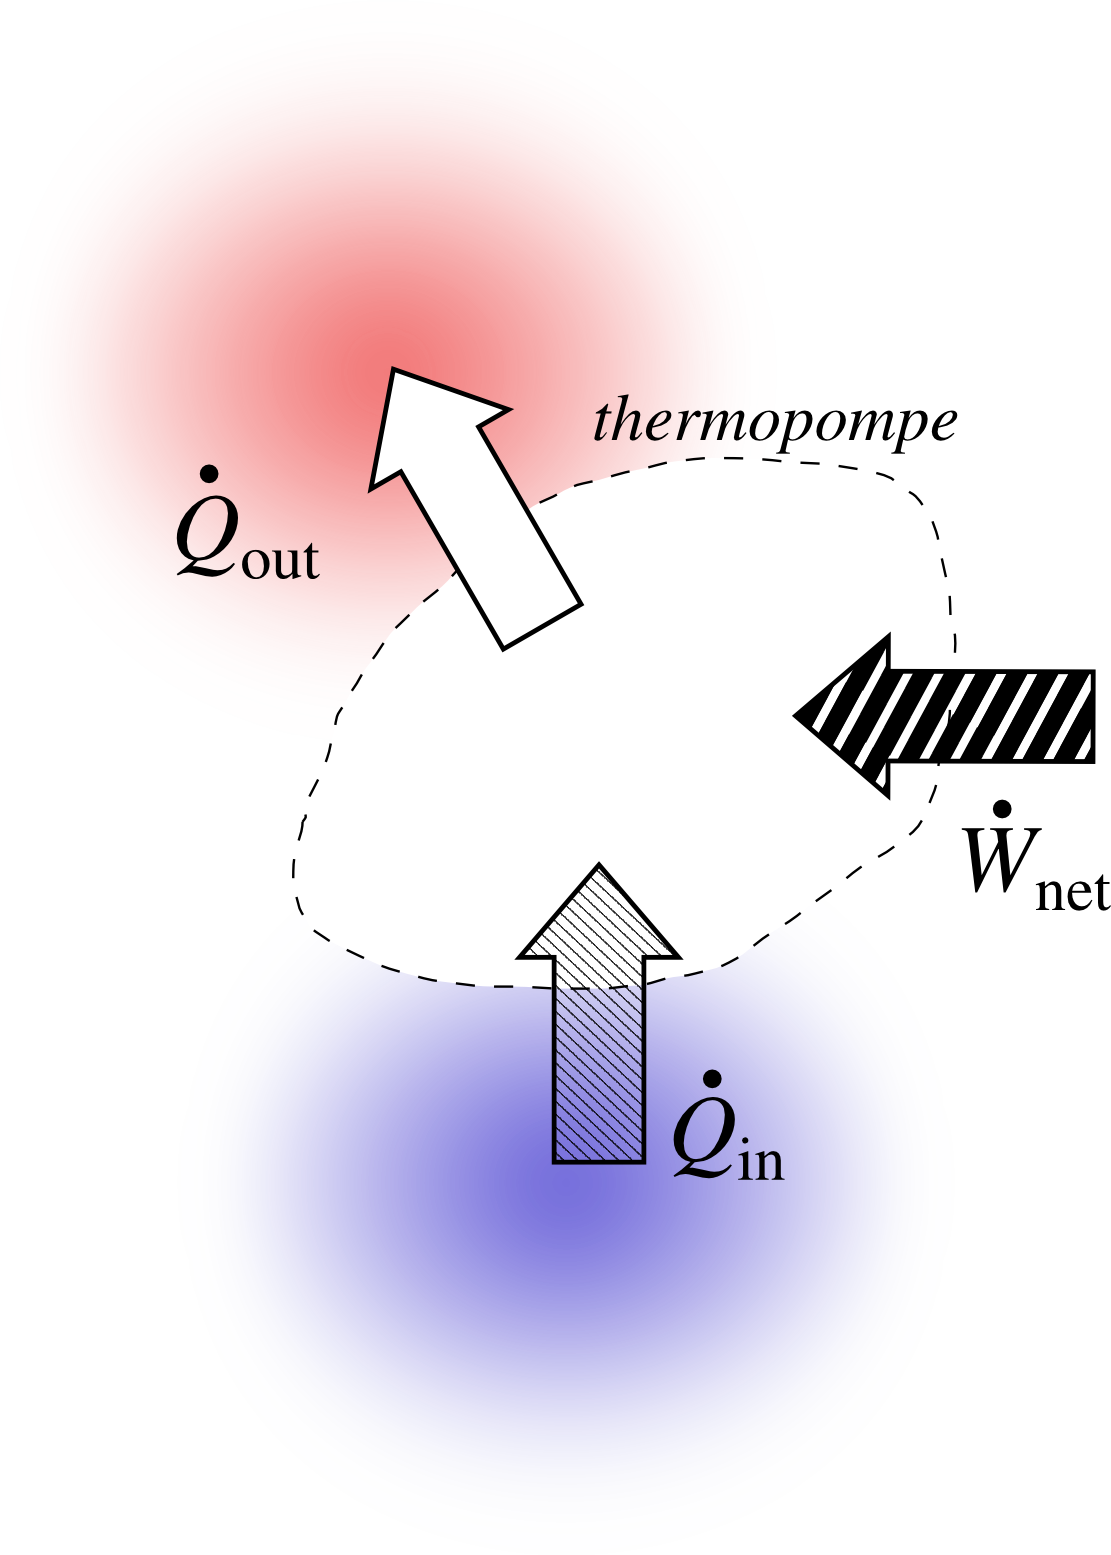
\includegraphics[width=6cm]{images/efficacite_thermopompe.png}
				\vspace{-1cm}
			\end{center}
			\supercaption{Transferts énergétiques associés à une pompe à chaleur.
					On souhaite obtenir un grand transfert $\dot Q_\out$ (résultat) à partir du transfert $\dot W_\net$ (coût).}{schéma \cczero \oc}
			\label{fig_transferts_thermopompe}
		\end{figure}

		\index{COP (coefficient of performance)}\index{coefficient of performance (COP)}
		Le rendement $\eta_\text{thermopompe}$ (dit aussi $\textsc{cop}_\text{thermopompe}$) de la thermopompe est donc défini par :
		\begin{equation}
			\eta_\text{thermopompe} \equiv \left| \frac{\dot Q_\out}{\dot W_\net} \right|
			\label{def_rendement_thermopompe}
		\end{equation}
	
			\begin{anexample}
				Une pompe à chaleur consomme une puissance électrique de~\SI{100}{\watt} ; elle chauffe l’intérieur d’une pièce avec une puissance de~\SI{350}{\watt}. Quel est son rendement ?
		
				\begin{answer}
					Le rendement est de $\eta_\text{thermopompe} = \left| \frac{\dot Q_\out}{\dot W_\net} \right| = \left| \frac{\num{-350}}{\num{+100}} \right| = \num{3.5}$.
						\begin{remark} La pompe à chaleur rejette plus de chaleur qu’elle ne consomme de travail –\ c’est tout son intérêt. Si le \textsc{cop} était égal ou inférieur à~\num{1}, il serait plus économique et bien plus simple d’utiliser un radiateur électrique.\end{remark}
				\end{answer}
			\end{anexample}


		De la même façon que pour les sections précédentes, on peut exprimer ce rendement en fonction des débits de chaleur uniquement :
		\begin{equation}
			\eta_\text{thermopompe} = \frac{1}{1 - \left| \frac{\dot Q_\inn}{\dot Q_\out} \right|}
			\label{eq_rendement_thermopompe_qin_qout}
		\end{equation}



	\onlyframabook{\clearpage}
	\subsection{De la faible performance des machines}\index{cycle!thermodynamique, faiblesse du rendement}

		\thermoquotebegin{O}
			L’on a souvent agité la question de savoir si la puissance motrice de la chaleur est limitée, ou si elle est sans bornes ; si les perfectionnements possibles des machines à feu ont un terme assignable, terme que la nature des choses empêche de dépasser par quelque moyen que ce soit, ou si au contraire ces perfectionnemens sont susceptibles d’une extension indéfinie…
		\thermoquoteend{Sadi Carnot, 1824~\cite{carnot1824}\cite{Carnot!Sadi}}{\onlyframabook{\vspace{-1em}}}

		Dans tous les cas que nous avons étudiés plus haut, pour chaque cycle, nous avons inclus un transfert indésirable. Dans le cycle moteur, une partie de l’énergie est gâchée sous forme de rejet de chaleur ($\dot Q_\out$). Dans les cycles de réfrigération, on doit apporter du travail ($\dot W_\inn$) pour effectuer un transfert de chaleur qui \textit{a priori} aurait pu sembler «~gratuit~» ($\dot Q_\out$ étant alors égal à $\dot Q_\inn$).

		L’étudiant/e en ingénierie s’indignera certainement de la place qu’occupent ces pertes dans ce chapitre --\ et des timides rendements atteints par les machines décrites en exemple. Pourquoi les rendements calculés dans les exemples et dans les exercices qui suivent sont-ils si faibles, et surtout, comment concevoir des cycles de plus grande efficacité ? Nous aurons soin et à cœur de répondre à ces questions au \courssept.
\index{cycle!thermodynamique|)textbf}
